\documentclass[preprint]{sigplanconf} % <<<

\usepackage{amsmath}
\usepackage{amssymb}
\usepackage{amsthm}
\usepackage{graphics}
\usepackage[latin1]{inputenc}
\usepackage{microtype}  % do not remove
\usepackage{pygmentize}
\usepackage{rgalg}
\usepackage{tikz}
\usepackage{xcolor}

\usepackage[colorlinks]{hyperref} % keep it last to avoid some warnings

\RecustomVerbatimEnvironment{Verbatim}{BVerbatim}{}
\definecolor{darkblue}{rgb}{0,0,0.4}
\definecolor{verylightgray}{rgb}{0.9,0.9,0.9}
% comment the next line for printing
\hypersetup{colorlinks,linkcolor=darkblue,citecolor=darkblue,urlcolor=darkblue}
\hypersetup{
  pdftitle={A Language for Specifying Safety Temporal Properties of Object-Oriented Programs},
  pdfauthor={Radu Grigore and Rasmus Lerchedahl Petersen and Dino Distefano}}

\titlebanner{DRAFT}
\title{TOPL: A Language for Specifying Safety Temporal Properties of Object-Oriented Programs}
\authorinfo{Radu Grigore \and Rasmus Lerchedahl Petersen \and Dino Distefano}{Queen Mary, University of London}{{\rm\{}rgrig,rusmus,ddino{\rm\}}@eecs.qmul.ac.uk}

% rg: I tend to give grammars in BFS order
\def\grammar#1{{
  \footnotesize
  \def\b##1{{\rm\Verb@##1@}}\def\*{$^*$}\def\?{$^?$}\def\({$($}\def\){$)$}
  \def\|{$\mid$}\def\+{$^+$}
  \smallskip
  \hbox to\hsize{\hfil\vbox{\halign{\hfil\it##&$\;::=\;$\it##\hfil&\qquad\rm##\hfil\cr#1}}\hfil}
  \smallskip
}}

\renewcommand{\sectionautorefname}{Section}
\renewcommand{\subsectionautorefname}{\sectionautorefname}

\newcommand{\dinocomment}[1]{
\begin{center}
\fbox{
\begin{minipage}{3.0in}
{\bf Dino's comment:} {\it #1}
\end{minipage}}
\end{center}}

\newcommand{\note}[2]{\textcolor{gray}{[\textcolor{red}{#1}: #2]}}
\newcommand{\rg}[1]{\note{rg}{#1}}

\newcommand{\N}{\ensuremath{\mathbb{N}}}
\newcommand{\eval}[1]{[[#1]]}
\newcommand{\pmap}{\rightharpoonup}
\newcommand{\set}[1]{\ensuremath{\mathsf{#1}}}
\newcommand{\verbline}[2][]{\[\text{\Verb@#2@}#1\]}
\newcommand{\TPL}{TOPL}

\theoremstyle{definition}
\newtheorem{example}{Example}

\overfullrule=5pt
\showboxdepth=10
\showboxbreadth=30
% >>>
\begin{document}
\maketitle

\begin{abstract} % <<<
In this paper we present ongoing work related to a new specification language for temporal safety properties aimed at object-oriented languages.
The language is expressive enough to represent relationships between objects and it is designed with the goal of performing dynamic and static analysis of object-oriented software.
\end{abstract}
\category{D.2.1}{Software Engineering}{Requirements/Specifications}
\terms Languages, Verification
\keywords Safety, Temporal Properties, Object-Oriented

% >>>
\section{Introduction} % <<<
One popular class of properties addressed by many techniques in program verification is to check whether a program satisfies some specified safety property.  
Violations of this class of properties may lead to unexpected run-time errors.

Many safety properties can be expressed using the framework of {\em typestate}~\cite{strom1986} which uses finite state automata for specifying conformance or violation w.r.t. a temporal safety property.
These properties are related with the correct use of types operations in different contexts. 
For example in object-oriented languages the correct use of the APIs of certain classes may be particularly 
delicate and it is easy for the programmer to break essential invariants.

The long term aim of our project is the automatic verification of typestate properties of Java programs of realistic size.  
The properties should be given by the user; they should not be hard-coded.
In order to achive our goal we would need
\begin{itemize}
\item A language for specifying temporal safety properties;
\item An automatic tool that can verify the properties in the language
  against Java programs.
\end{itemize}
This paper addresses the first point by introducing \TPL  \ (Temporal Object Property Language, pronounced like `topple').
It has the following characteristics:
\begin{itemize}
\item It is designed specifically for expressing properties of object-oriented software. For this reason \TPL \ allows expressing relations between object references.
%And since object-oriented languages like Java make heavy use of the heap, we have designed our language based on separation logic~\cite{reynolds2002} a formalism known to be effective and concise in specifying heap related properties.
%\rg{I would not mention separation logic here.
%We did not quite get to using it, although that's what we want for TACAS\null.
%It might look like some gratuitous `name-dropping'.
%The Future Work or the Conclusions sections are better places.}
\item It allows very high-level intuitive specifications my means of automata tailored towards object-oriented specifications.
\item It is designed to be used to do program analysis (both static and dynamic).
\end{itemize}  
In this paper we introduce \TPL \ and its formal semantics. 
Moreover we show its use for dynamic checking of the properties against  a simple object-based language. 
One of the advantage of dynamic checking w.r.t. using exceptions in the Java code is that it is possible to return a trace to the programmer. 
Traces of events triggering an error are extremely useful for debugging purposes.
Moreover, writing code for checking that a property is violated can be complex and error prone. It simple distracts the programmer from the core algorithmic problems that is trying to solve.




% contributions
% - language for temporal properties
% - keep references (object) relationship
% - designed for oop
% - designed for doing analysis (dyn/stat)
% - High-level/simple
% Safety (obiquitus)

The paper is organized as follows. In Section~\ref{sec:example} we start with a motivating example. 
Section~\ref{sec:syntax} gives the syntax of \TPL \ and in Section~\ref{sec:semantics} introduces its semantics. 
Section~\ref{sec:testing} describes the use of \TPL \ for run-time checking of safety properties. 
Section~\ref{sec:related} discusses related work and our future plans. 
Finally, Section~\ref{sec:conclusions} conclude the paper.
% >>>
\section{Examples} \label{sec:example} % <<<

The first example (\autoref{sec:example.steps}) is a fairly subtle property imposed on the users of the Java~API which causes trouble in practice from time to time.
It is sufficiently complex to illustrate a large part of our language.
Properties are essentially automata that monitor program executions.
For this first example we illustrate the semantics of the automaton by going step-by-step through an execution.

The following examples (\autoref{sec:example.others}) illustrate the expressivity of the property language.

\subsection{Invalidating Iterators} \label{sec:example.steps} % <<<

The last statement in \autoref{fig:running.java} throws an exception.
There are two iterators on the same collection, one of them modifies the collection, and this invalidates the other iterator.
The automaton in \autoref{fig:running.drawing} formally captures the disallowed API usage.
The automaton is essentially depicted  in a graphical form, whereas  \autoref{fig:running.property} shows the same automaton (in \TPL ) given  as a list of labeled transitions. 
Each label is a statement pattern.
 

\begin{figure} % running example <<<
\begin{Verbatim}[commandchars=\\\{\}]
\PY{k+kn}{import} \PY{n+nn}{java.util.*}\PY{o}{;}
\PY{k+kd}{public} \PY{k+kd}{class} \PY{n+nc}{IncorrectIteratorUse} \PY{o}{\PYZob{}}
  \PY{k+kd}{public} \PY{k+kd}{static} \PY{k+kt}{void} \PY{n+nf}{main}\PY{o}{(}\PY{n}{String}\PY{o}{[}\PY{o}{]} \PY{n}{args}\PY{o}{)} \PY{o}{\PYZob{}}
    \PY{n}{List}\PY{o}{<}\PY{n}{Integer}\PY{o}{>} \PY{n}{c} \PY{o}{=} \PY{k}{new} \PY{n}{ArrayList}\PY{o}{<}\PY{n}{Integer}\PY{o}{>}\PY{o}{(}\PY{o}{)}\PY{o}{;}
    \PY{n}{c}\PY{o}{.}\PY{n+na}{add}\PY{o}{(}\PY{l+m+mi}{1}\PY{o}{)}\PY{o}{;} \PY{n}{c}\PY{o}{.}\PY{n+na}{add}\PY{o}{(}\PY{l+m+mi}{2}\PY{o}{)}\PY{o}{;}
    \PY{n}{Iterator}\PY{o}{<}\PY{n}{Integer}\PY{o}{>} \PY{n}{i} \PY{o}{=} \PY{n}{c}\PY{o}{.}\PY{n+na}{iterator}\PY{o}{(}\PY{o}{)}\PY{o}{;}
    \PY{n}{Iterator}\PY{o}{<}\PY{n}{Integer}\PY{o}{>} \PY{n}{j} \PY{o}{=} \PY{n}{c}\PY{o}{.}\PY{n+na}{iterator}\PY{o}{(}\PY{o}{)}\PY{o}{;}
    \PY{n}{i}\PY{o}{.}\PY{n+na}{next}\PY{o}{(}\PY{o}{)}\PY{o}{;} \PY{n}{i}\PY{o}{.}\PY{n+na}{remove}\PY{o}{(}\PY{o}{)}\PY{o}{;} \PY{n}{j}\PY{o}{.}\PY{n+na}{next}\PY{o}{(}\PY{o}{)}\PY{o}{;}
  \PY{o}{\PYZcb{}}
\PY{o}{\PYZcb{}}
\end{Verbatim}

\caption{Running example: Java code}
\label{fig:running.java}
\end{figure}
\begin{figure}
\begin{Verbatim}
property InvalidateOtherIterators
  using prefix java.util.Collection
  using prefix java.util.Iterator
  start -> gotOne:    I := C.iterator()
  gotOne -> gotTwo:   J := c.iterator()
  gotTwo -> jInvalid: i.remove()
  gotTwo -> iInvalid: j.remove()
  jInvalid -> error:  call j.*[*]
  iInvalid -> error:  call i.*[*]
\end{Verbatim}
\caption{Running example: Safety property}
\label{fig:running.property}
\end{figure}
\begin{figure}
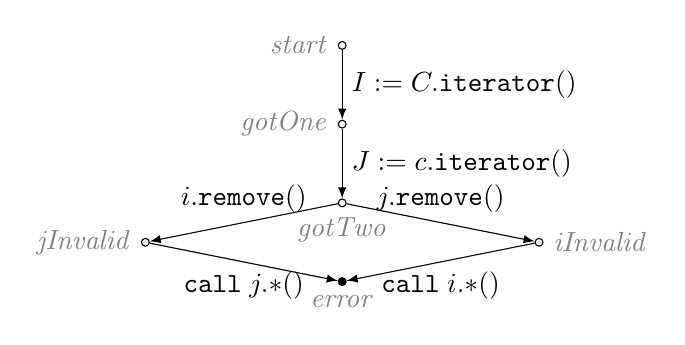
\begin{tikzpicture}[xscale=2.5]
  \tikzset{vertex/.style={draw,circle,inner sep=1pt}}
  \tikzset{transition/.style={->,>=latex}}
  \tikzset{every label/.style={gray}}
  \node[vertex] (start) at (0,0) [label=left:\textit{start}] {};
  \node[vertex] (gotOne) at (0,-1) [label=left:\textit{gotOne}] {};
  \node[vertex] (gotTwo) at (0,-2) [label=below:\textit{gotTwo}] {};
  \node[vertex] (iInvalid) at (1,-2.5) [label=right:\textit{iInvalid}] {};
  \node[vertex] (jInvalid) at (-1,-2.5) [label=left:\textit{jInvalid}] {};
  \node[vertex,fill] (error) at (0,-3) [label=below:\textit{error}] {};
  \draw[transition] (start)--node[right]{$I:=C.\mathtt{iterator}()$} (gotOne);
  \draw[transition] (gotOne)--node[right]{$J:=c.\mathtt{iterator}()$} (gotTwo);
  \draw[transition] (gotTwo) -- node[above]{$j.\mathtt{remove}()$} (iInvalid);
  \draw[transition] (gotTwo)--node[above]{$i.\mathtt{remove}()$} (jInvalid);
  \draw[transition] (iInvalid)--node[below]{$\mathtt{call}\;i.{*}()$} (error);
  \draw[transition] (jInvalid)--node[below]{$\mathtt{call}\;j.{*}()$} (error);
\end{tikzpicture}
\caption{Running example: Drawing of safety property}
\label{fig:running.drawing}
\end{figure}
\begin{figure}
\begin{align*}
&\{(\mathit{start}, [])\} \\
&\text{\Verb+\PY{n}{Iterator}\PY{o}{<}\PY{n}{Integer}\PY{o}{>} \PY{n}{i} \PY{o}{=} \PY{n}{c}\PY{o}{.}\PY{n+na}{iterator}\PY{o}{(}\PY{o}{)}\PY{o}{;}+} \\
&\text{assume $c$ holds $1$, and $i$ holds $2$ } \\
&\{(\mathit{start},[]), (\mathit{gotOne},[c:1, i:2])\} \\
&\text{\Verb+\PY{n}{Iterator}\PY{o}{<}\PY{n}{Integer}\PY{o}{>} \PY{n}{j} \PY{o}{=} \PY{n}{c}\PY{o}{.}\PY{n+na}{iterator}\PY{o}{(}\PY{o}{)}\PY{o}{;}+}\\
&\text{assume $j$ holds $3$} \\
&\{(\mathit{start},[]), (\mathit{gotOne},[c:1,i:3]),(\mathit{gotTwo},[c:1,i:2,j:3])\} \\
&\text{\Verb+\PY{n}{i}\PY{o}{.}\PY{n+na}{next}\PY{o}{(}\PY{o}{)}\PY{o}{;}+} \\
&\{(\mathit{start},[]), (\mathit{gotOne},[c:1,i:3]),(\mathit{gotTwo},[c:1,i:2,j:3])\}\\
&\text{\Verb+\PY{n}{i}\PY{o}{.}\PY{n+na}{remove}\PY{o}{(}\PY{o}{)}\PY{o}{;}+} \\
&\{(\mathit{start},[]), (\mathit{gotOne},[c:1,i:3]),(\mathit{jInvalid},[c:1,i:2,j:3])\} \\
&\text{\Verb+\PY{n}{j}\PY{o}{.}\PY{n+na}{next}\PY{o}{(}\PY{o}{)}\PY{o}{;}+}\\
&\{(\mathit{start},[]), (\mathit{gotOne},[c:1,i:3]), (\mathit{error},[c:1,i:2,j:3])\}
\end{align*}
\caption{Running example: Step by step}
\label{fig:running.steps}
\end{figure} % >>>

\autoref{fig:running.steps} shows how an execution of the program drives the automaton.
The automaton is nondeterministic so it has a \emph{set} of active states.
Initially, only the state $(\mathit{start},[])$ is active.
The outgoing transition of vertex \textit{start} is labeled by \[I:=C.\mathtt{iterator}()\] and the statement about to be executed is \verbline[.]{i = c.\PY{n+na}{iterator}()}
To see if the pattern matches the statement we first look at the method.
For simplicity, we identify Java methods by their fully qualified names and their arities.
In this case, the method that is invoked is \verbline[.]{java.util.ArrayList.iterator[1]}
The \texttt{using prefix} directives say that the string \texttt{iterator} appearing in the automaton label is a shorthand for one of two method names.
The pattern matches the methods
\begin{align*}
&\text{\Verb@java.util.Collection.iterator[1]@} \\
&\text{\Verb@java.util.Iterator.iterator[1]@}
\end{align*}
and all the methods that override them.
In this case, the \textit{iterator} method in \textit{ArrayList} overrides the one in \textit{Collection} so we have a match.
Next, we look at the patterns $I$~and~$C$.
By convention, patterns starting with an uppercase letter match any \emph{value}.
In this case, they match the values held by the program variables $i$~and~$c$.
At this point, all conditions are met to perform the transition from \textit{start} to \textit{gotOne}.
Performing a transition involves remembering the values on which the uppercase patterns matched.
For concreteness, let us assume that the program variables $c$~and~$i$ hold the values $1$~and~$2$.
Then, performing the first transition stores the values $1$~and~$2$ into the \emph{automaton variables} $c$~and~$i$.
\dinocomment{I get confused why we need to specify that $c$ and $i$ holds 1 and 2. Or maybe I don't understand why do we need to talk about the value of $c$ and $i$ at this point....}
The automaton variables live in a different name-space from program variables.
In this case we use the same names for automaton variables as for program variables purely as a mnemonic device---there is no semantics to it.
The end result of performing the transition from \textit{start} to \textit{gotOne} is that the state \[(\mathit{gotOne},[c:1,i:2])\] is activated.
Usually, the source of a transition would not be active anymore.
In this case, the state $(\mathit{start},[])$ remains active because it is a special state that is always active.
Conceptually, the vertex \textit{start} has a self-loop on it that always matches.

For the second step we need to consider the two active states in turn.
For $(\mathit{start},[])$ exactly the same reasoning holds and the result is that \[(\mathit{gotOne},[c:1,i:3])\] is active after the second step.
Note that now the automaton variable~$i$ remembers the value of the program variable~$j$.
For \[\mathit{gotOne},[c:1,i:2])\] we look at the transition outgoing from vertex \textit{gotOne}.
It has the label \[J:=c.\mathtt{iterator}();\]
the statement to be executed is \verbline[.]{j = c.\PY{n+na}{iterator}()}
The method and the uppercase pattern~$J$ match in the same way as before.
The lowercase pattern $c$ matches only the value that is held by the automaton variable~$c$.
In summary, uppercase patterns write to the automaton memory, and lowercase patterns read from the automaton memory and act as a guard on the transition.
In this case, the transition $\mathit{gotOne}\to\mathit{gotTwo}$ is performed because the program variable~$c$ still refers to the same collection it did when the transition $\mathit{start}\to\mathit{gotOne}$ was performed.

In the third step, no transition is performed and the same states remain active.
None of the outgoing transitions of \textit{start}, \textit{gotOne}, and \textit{gotTwo} match the method \textit{next}.
\dinocomment{So I guess we should explain that the program progresses whereas the automaton wait. It's a bit strange so better to explicitly say}

In the fourth step, the transition $\mathit{gotTwo}\to\mathit{jInvalid}$ is performed.
The pattern $i.\mathtt{remove}()$ does not have a left-hand side, which simply means that the returned value does not matter.
The states corresponding to vertices \textit{start} and \textit{gotOne} remain unchanged, because their outgoing transitions do not match.

For the fifth and final step, one of the active states is \[(\mathit{jInvalid},[c:1,i:2,j:3]),\] the label on its outgoing transition is \[\mathtt{call}\;j.{*}(),\] and the statement to be executed is \verbline[.]{j.\PY{n+na}{next}()}
The pattern has two distinguishing features, the~$*$ as a method name and the tag \texttt{call}.
Let us discuss first the method name.
\rg{TODO: Explain the arity notation [$n$].}
\rg{TODO: Say that the lack of return (or arguments) means ``anything matches.''}
As before, the first step is to prepend the prefixes.
\begin{align*}
&\text{\Verb@java.util.Collection.*[*]@} \\
&\text{\Verb@java.util.Iterator.*[*]@}
\end{align*}
Next, the $*$s are expanded, taking into account the \texttt{CLASSPATH}.
We have a match because the expansion \verbline{java.util.Iterator.next} is overridden by the method that is actually called.

The \texttt{call} tag touches on a subtle part of the semantics that will be fully explained later (\autoref{sec:semantics}).
Note that a pattern like $I:=C.\mathtt{iterator}()$ conceptually refers to \emph{two} moments in time---the call time and the return time.
In particular, in-between those two events other methods might be called.
A simple way to disambiguate what is meant is to prepend the label with the tag \texttt{call} or the tag \texttt{return}.
When the tag is \texttt{call}, there can be no left-hand side;
when the tag is \texttt{return}, the right-hand side is only a method name pattern.
Here is an example of a return transition \verbline[.]{x -> y: return I := iterator[1]}
If a tag is not present, then the transition is said to be a \emph{call--return transition}.
We allow the user to use such transitions for convenience.
Roughly speaking, we require the call and the return events of a call--return transition to be consecutive.

The execution we stepped through violates the property \textit{InvalidateOtherIterators} because the vertex \textit{error} is reached.
Notice that in order to find a counterexample we need to keep track of the relation between several objects: ``these two iterators are for the same collection.''
In practice, programmers tend to violate this property when the code is more involved and uses the shorthand notation for iteration $\mathbf{for}(T\;x:c)$.

\paragraph{Discussion.}
How is this better than just having an exception thrown by the Java~API\null?
\begin{itemize}
\item We can record which statements trigger which transitions, so we can have a trace that explains what exactly went wrong.
\item We do not need to write the code that checks whether the property is violated.
  In this example, the programmers of the Java standard libraries hand-coded the check that throws an exception.
  The check involves storing some extra state in collections, is fairly complicated, and therefore error-prone itself.
  By comparison, the code in \autoref{fig:running.property} is simple and captures how programmers think about the property.
\item One can retro-actively document third-party libraries with such properties without having access to the code.
\item It is possible in principle to design a static analysis for such properties.
  In fact, designing a static analysis is our goal and the original motivation for designing this property language.
  Our current prototype only does run-time checking, though.
\end{itemize}

Are there any disadvantages?
Yes, a big disadvantage is that checking an arbitrary property involves keeping track of a potentially unbounded number of states.
For particular properties, programmers can specialize the check and make it more efficient.

% >>>
\subsection{Other Examples of Typestate-like properties in \TPL} \label{sec:example.others} % <<<
A property closely related to \autoref{fig:running.property} is that 
{\it modifying the collection directly invalidates all iterators.}
%
In \TPL \ this  property can be expressed as follows:
%
\par\medskip\noindent
\begin{Verbatim}
property ModificationInvalidatesIterators
  using prefix java.util.{Collection,Iterator}
  start -> iterating:     I := C.iterator()
  iterating -> modified:  c.add(*), c.remove(*)
  modified -> error:      call i.*[*]
\end{Verbatim}
\par\medskip\noindent This property should list all the methods of \textit{Collection} that mutate it.
If classes that implement \textit{Collection} add mutating methods, then those should be included as well.
This ``abstraction leak'' is intrinsic to Java where sub-classing is not sub-typing.

Another property related to iterators, is that {\it iterators should not be advanced unless we know that they are not exhausted.} 
In \TPL:
\par\medskip\noindent
\begin{Verbatim}
property UnsafeIteratorNext
  using prefix java.util.{Collection,Iterator}
  start -> iterating:         I := *.iterator()
  iterating -> notExhausted:  true := i.hasNext()
  notExhausted -> iterating:  i.next()
  iterating -> error:         i.next()
\end{Verbatim}
\par\medskip

\paragraph{Temporal properties of resources.}
Many resources impose a temporal property:
Before being used they must be acquired;
after being used they must be released.
Examples include memory allocation and deallocation, locks for synchronization between threads, opening and closing files, and establishing and closing network connections.
The liveness property, which we do not handle, is that each \textit{acquire} is eventually followed by a \textit{release}.
However, ignoring programs that run forever this property can be rephrased as a safety property:
When the program terminates, the last action must have been \textit{release}.
\dinocomment{Really should be the last action?}
Suppose that resources are represented by instances of the class \textit{Resource}, which has two methods, \textit{acquire} and \textit{release}.
\par\medskip\noindent
\begin{Verbatim}
property ResourceLeak
  start -> released:    R := new Resource()
  released -> acquired: r.acquire()
  acquired -> released: r.release()
  acquired -> error:    return Main.main(*)
\end{Verbatim}
\par\medskip\noindent
Even without restricting our attention to terminating programs there are two other safety properties that are imposed:
there should be no two consecutive \textit{acquire} or two consecutive \textit{release}.
\par\medskip\noindent
\begin{Verbatim}
property DoubleAcquireOrRelease
  start -> released:    R := new Resource()
  released -> acquired: r.acquire()
  acquired -> released: r.release()
  released -> error:    r.release()
  acquired -> error:    r.acquire()
\end{Verbatim}
\par\medskip\noindent
Normally this automaton would be split into two so that error messages are more informative and precise.

\paragraph{Immutable data structures.}
Another common issue in Java is providing read-only access to collections.
For example, if one wants to implement an immutable data structure, the common idiom is to make all fields private, provide getter, but not setters.
However, if deep-immutability is desired and one of the members is a collection, then extra precautions are necessary.
One solution is to use third-party immutable collections.
Another solution is to make a copy of the collection in the getter.
Another solution is to return an unmodifiable view.
\rg{TODO: Read the API carefully and see how this works.
I remember that the guava guys said this solution doen't really work, but I don't remember why.
If it \emph{does} work, then there's not much point to give this example.
Except, perhaps, that you can verify (or rather test) existing code.}
Yet another solution is to ask in comments to not modify collections obtained using a certain getter.
This last solution is good from a performance point of view.
It is also used in practice.
(See, for example, the class \textit{ComponentHelper} in Ant and its method \textit{getRestrictedDefinitions}.)
\par\medskip\noindent
\begin{Verbatim}
property ModifiedReadOnlyView
 using prefix org.apache.tools.ant.ComponentHelper
  start -> got: C := *.getRestrictedDefinitions()
  got -> error: c.add(*), c.remove(*)
  got -> iterating: I := c.iterator()
  iterating -> error: i.remove()
\end{Verbatim}
\par\medskip\noindent
\rg{TODO: Oops: the example above is wrong.
It's the second hint I get that we need a pattern for \textbf{this}.
The other was an example in Disney et al.
The idea is that it matters \emph{who} calls a certain method.
In this case, the \textit{ComponentHelper} itself \emph{is} allowed to modify the collection, but the property above will signal it as a violation.}

\rg{TODO: Add more examples here, preferably inspired by real code.
Also, add examples from Disney et al.}

\rg{TODO: See which bugs found by FindBugs can be expressed in our language.}

% >>>
% >>>
\section{Syntax}\label{sec:syntax} % <<<

We begin the systematic presentation of TOPL with its syntax (\autoref{sec:syntax.topl}).
Before moving on to semantics (\autoref{sec:semantics}) we shall also introduce the syntax of SOOL, a \textbf simple \textbf object-\textbf oriented programming \textbf language (\autoref{sec:syntax.sool}).
Our prototype implementation is an interpreter for SOOL programs that dynamically checks TOPL properties.

\subsection{TOPL and iTOPL}\label{sec:syntax.topl} % <<<

% plan
% - two languages
% - language for users
% - language for semantics
% - desugaring translation

TOPL aims to be intuitive:
Labels look like method calls, there is a shorthand notation for parallel transitions, there is an implied loop on the vertex \textit{start}, the \texttt{using prefix} directive offers some extra convenience, and so on.
From the point of view of semantics, however, these conveniences are in the way.
For this reason we also define iTOPL (\textbf inner TOPL), an even simpler language into which TOPL is desugared.

\autoref{fig:syntax.topl} shows the syntax of TOPL\null.
A property has a name, a set of \texttt{using} directives, and a set of transitions.
Each transition has an arc (directed edge) and labels.
Each arc has a source vertex and a target vertex.
All vertices are identified by their name.
Labels look roughly like method calls.
Each label has a method pattern that is used to identify the set of methods to which the label refers.
In the simple case, a method pattern consists of a string pattern for the name of the method and an integer that specifies the method arity.
(For simplicity, TOPL does not use the static types of arguments to distinguish between overloaded methods.)
The more interesting case is when there are value patterns for each argument and perhaps even for the context and the result.
The context pattern appears \Verb@<@surrounded by angle brackets\Verb@>@ at the beginning of the label and is matched against the value of the special variable \textbf{this}.
Transitions should typically be tagged with \texttt{call} or \texttt{return} to specify exactly at what time they should be performed (see \autoref{sec:semantics.topl} for details).

\begin{figure}
\grammar{
  Property& \b{property} Identifier Using\* Transition\* \cr
  Using& \b{using prefix} StringPattern \cr
  Transition& Arc \b: Label \(\b, Label\)\* \cr
  StringPattern& \(Letter \| \b. \| \b*\)\+ \cr
  Arc& Vertex \b{->} Vertex \cr
  Label& Context\? Tag\? MethodPattern \cr
  Vertex& Identifier \cr
  Context& \b< ValuePattern \b> \cr
  Tag& \b{call} \| \b{return} \cr
  MethodPattern& ResultPattern\? NamePattern ArgumentsPattern \cr
  ResultPattern& ValuePattern \b{:=} \cr
  NamePattern& StringPattern \cr
  ArgumentsPattern& \b( \(ValuePattern \(\b, ValuePattern\)\*\)\? \b) \cr
  ArgumentsPattern& \b[ IntegerPattern \b] \cr
  ValuePattern& \b* \| Literal \| UppercaseId \| \b!\? LowercaseId \cr
  IntegerPattern& \b* \| IntegerLiteral \cr
}
\caption{Syntax of TOPL}
\label{fig:syntax.topl}
\end{figure}

There are three types of patterns used in TOPL---for strings, for integers, and for values.
String patterns match method names and may use wildcards.
(For simplicity, TOPL does not use full regular expressions as string patterns.)
Integer patterns specify method arities.
Value patterns are the most interesting.
\rg{TODO: Explain wildcard and literals for value patterns.}
For each automaton variable \Verb@var@ there are three associated patterns.
The uppercase pattern \Verb@Var@ matches any value and writes it in the automaton variable \Verb@var@.
The lowercase pattern \Verb@var@ reads the value of the automaton variable \Verb@var@ and only matches that value.
The negated lowercase pattern \Verb@!var@ reads the value of the automaton variable \Verb@var@ and only matches different values.

A TOPL property is \emph{well-formed} when it satisfies the following conditions.
\begin{itemize}
\item Labels must contain uppercase value patterns at most once.
\item Any use of a lowercase patterns must be definitely preceded the corresponding uppercase pattern.
  In other words, automaton variables must be written before being read.
\end{itemize}

\autoref{fig:syntax.itopl} shows the syntax of iTOPL\null.
The missing productions are the same as for TOPL\null.
Each transition now has exactly one label.
Each label is a list of (guard, action) pairs.
Each guard is some boolean combination of atomic guards.
Each action is a sequence of atomic actions.
Both guards and actions refer to some implicit array of values using an index (see \autoref{sec:semantics.topl}).
Atomic guards compare values either with automaton variables (\textit{Identifier}) or with constants (\textit{Literal}).
Atomic actions write values into automaton variables.
There is also an atomic guard that matches against method calls and always specifies a tag \Verb@call@ or \Verb@return@, but never involves examining any values.

\begin{figure}
\grammar{
  Property& \b{property} Identifier Transition\* \cr
  Transition& Arc \b: Label \cr
  Label& \(\b(Guard Action\b)\)\* \cr
  Guard& AtomicGuard \| Guard \(\(\b{\&}\|\b|\) Guard\)\* \cr
  Action& \(AtomicAction \(\b, AtomicAction\)\*\)\? \cr
  AtomicGuard& \b! Guard \cr
  AtomicGuard& \b[ ValueIndex \b] \b= \(Identifier \| Literal\)\cr
  AtomicGuard& \(\b{call} \| \b{return}\) NamePattern \b[ IntegerPattern \b] \cr
  AtomicGuard& \b{true} \cr
  AtomicAction& Identifier \b{:=} \b[ ValueIndex \b] \cr
  ValueIndex& IntegerLiteral \cr
}
\caption{Syntax of iTOPL}
\label{fig:syntax.itopl}
\end{figure}

\rg{TODO: Present desugarings---things like methods names, going from patterns to guards and actions.}

% >>>
\subsection{SOOL}\label{sec:syntax.sool} % <<<

SOOL is a subset of existing object-oriented languages.
It has classes, assignments, and method calls.
It should be possible to use TOPL with any language that is a superset of SOOL\null.
\rg{TODO: rewrite and continue}

\begin{figure}
\grammar{
  Program& \(Class \| VarDecl\)\* Main\cr
  Class& \b{class} Identifier Member\* \cr
  VarDecl& \b{var} Type Identifier \cr
  Main& \b{main} Body \cr
  Member& VarDecl &field \cr
  Member& Type Identifier \b( Arguments\? \b) Body & method\cr
  Body& VarDecl\* Statement\* \cr
  Arguments& Type Identfier \(\b, Type Identifier\)\* \cr
  Statement& \b{return} Expression & return\cr
  Statement& Identifier \b{:=} \b{new} & allocate \cr
  Statement& Identifier \b{:=} Expression & assign \cr
  Statement& \(Identifier \b{:=}\)\? Expression \b. Identifier & call \cr
  Statement& \(\b{do} Body\)\? \b{while} Expression Body\? &loop\cr
  Statement& \b{if} Expression Body \(\b{else} Body\)\? &test\cr
}
\caption{(Partial) Syntax of SOOL}
\label{fig:syntax.sool}
\end{figure}

% >>>
% >>>
\section{Semantics}\label{sec:semantics} % <<<

A program's semantics is a set of event traces;
an automaton's semantics is also a set of event traces.
If the automaton express undesired behaviour, then a program \emph{violates} a property when their sets intersect.
Both the program and the automaton are nondeterministic.
%\dinocomment{So we only want to use the automata to specify bad behaviour?
%How about good behaviour?
%\rg{Ignoring the loop on \textit{start}, I think that every `good property' can be negated and converted into a negative one.
%You turn the accepting state into a stuck state and you add an error state that has incoming transitions from all normal states.
%These incoming transitions are tagged with the `end of execution' event.}}

\subsection{Automaton}\label{sec:semantics.topl} % <<<

Each event has a tag and carries an array of values.
\begin{align}
\set{Event}&=\bigcup_{n\in\N}\set{Tag}_n\times(n\to\set{Value})
\end{align}
(As usual, $n=\{0,1,\ldots,n-1\}$.)
The content of the undefined sets (such as \set{Value}) is not important.
We assume that these basic sets are disjoint.
Traces are finite.
\begin{align}
\set{Trace}=\bigcup_{n\in\N} n\to\set{Event}
\end{align}
Intuitively, the program outputs a trace that drives the automaton.

The automaton is defined on top of a finite multi-graph.
The automaton is an array of transitions.
Each transition has an edge and an array of labels.
Each edge has a source vertex and a target vertex.
Each label is a (guard, action) pair.
There are at least two vertices.
\begin{align}
\set{Automaton} &= \bigcup_{n\in\N} n \to \set{Transition} \\
\set{Transition} &= \set{Edge}\times \bigcup_{n\in\N} n\to\set{Label} \\
\set{Edge}&=\set{Vertex}\times\set{Vertex} \\
\set{Label}&=\set{Guard}\times\set{Action} \\
\{\mathtt{start},\mathtt{error}\}&\subseteq\set{Vertex}
\end{align}
The deterministic state contains a store of values.
\dinocomment{this deterministic state seems to come out of the blue.
\rg{What do you mean?
This is its definition.}}
\dinocomment{I think it would be good to give an introduction about the determinist state. What is it? Why it is needed?
etc. Just the definition at this point leave the reader wondering...}
A store is a finite partial map from automaton variables to values.
We also define an automaton deterministic execution state, which includes the input to be processed.
\begin{align}
\set{Store}&=\set{Variable}\pmap\set{Value} \\
\set{AState}&=\set{Vertex}\times\set{Store} \\
\set{EAState}&=\set{AState}\times\set{Trace}
\end{align}
Guards compare the values in an event with those in a store.
Actions modify the store, using values from an event.
\begin{align}
\set{Guard}&=\set{Event}\to\set{Store}\to2 \\
\set{Action}&=\set{Event}\to\set{Store}\to\set{Store}
\end{align}
The automaton deterministic step function evolves the execution state.
\begin{align}
\mathit{adStep}\in\set{EAState}\to\set{EAState}\to2
\end{align}
\begin{example}
Consider an automaton in state~$s_1$.
The input is a trace~$e_1e_2$ obtained by concatenating traces $e_1$~and~$e_2$.
The automaton must make a nondeterministic choice out of some alternatives.
A feasible alternative might be to consume $e_1$ and move to state~$s_2$.
For this, we write $(s_2,e_2)\in\mathit{adStep}(s_1,e_1e_2)$.
(We write $x\in f$ to mean that $f(x)=1$.)
\end{example}
The nondeterministic step is defined in terms of~\textit{adStep}.
\begin{align}
\mathit{anStep}&\in(\set{EAState}\to2)\to\set{EAState}\to2 \\
\mathit{anStep}\;S&=\bigcup \mathit{map}\;\mathit{adStep}\;S
\end{align}
An iterated version of \textit{anStep} is useful for defining reachable states.
We define it as the least fixed point for the following equation.
\begin{align}
\mathit{anStep}^\star\;S &= S \cup \mathit{anStep}^\star\;(\mathit{anStep}\;S)
\end{align}
Finally, we can define the set of traces described by an automaton.
\[ \{ e \mid \exists\sigma'e',\;((\mathtt{error},\sigma'),e')\in\mathit{anStep}^\star\;\{((\mathtt{start},0),e)\}\} \]
These are the traces that drive the automaton from the \texttt{start} vertex (with an empty store) to the \texttt{error} vertex.

\autoref{fig:adStep} defines \textit{adStep}.
Consider an automaton in state~$(x_1,\sigma_1)$ that processes trace~$e_1$.
If there is a transition from~$x_1$ to~$x_2$ that matches the events in a prefix~$e$ of~$e_1$, then the automaton may nondeterministically choose to perform that transition (line~10).
If no such transition exists, then the first event in $e_1$ is dropped and the automaton remains in the same state (line~11).
The actions of a transition are performed in order.
The guards are evaluated after all previous actions were performed.
A transition matches when all its guards hold.

\begin{figure}
\hbox to\hsize{\vbox{
\begin{alg}
\^  $\proc{adStep}\;((x_1,\sigma_1),e_1)\;((x_2,\sigma_2),e_2)$
\=  ~if~ $e_2$ is not a suffix of $e_1$ ~then return~ $0$
\=  $e:=\text{$e_1$ without the suffix $e_2$}$
\=  ~for each~ transition $((y_1,y_2),l)$
\+    ~if~ $(y_1,y_2)\ne(x_1,x_2) \lor \mathit{len}\;l\ne\mathit{len}\;e$ ~then continue~
\=    $\sigma:=\sigma_1$
\=    ~for each~ $k\in\mathit{len}\;l$
\+      $(g,a):=l\;k$
\=      ~if~ $\lnot(g\;(e\;k)\;\sigma)$ ~then continue~ to line 3
\=      $\sigma:=a\;(e\;k)\;\sigma$
\-    ~if~ $\sigma=\sigma_2$ ~then return~ $1$
\-  ~return~ $\mathit{len}\;e=1\land\sigma_1=\sigma_2$
\end{alg}
\smallskip
}\hfil}
\caption{One automaton step}
\label{fig:adStep}
\end{figure}

The function~\textit{adStep} is the crux of the automata semantics.
At line~5 a copy of the store is made, which is used by the following loop.
This copy is how \emph{roll-back} is built into the semantics of the automata.
If transitions always have length~$1$, then \textit{adStep} becomes simpler.
However, we could not find a desugaring into automata with transitions of length~$1$.

% >>>
\subsection{Program} % <<<

Let us now see how a simple object-oriented language produces event traces.
The state of the program is the content of the memory.
The program store (also known as stack) is similar to the automaton store.
Program variables and automaton variables live in different name-spaces.
Heaps map object addresses and field names to their values.
\begin{align}
\set{PState}&=\set{Store}\times\set{Heap}\\
\set{Heap}&=(\set{Value}\times\set{Variable})\pmap\set{Value}
\end{align}
The input is an array of values.
The program execution state keeps track of the input yet to be processed.
\begin{align}
\set{Input}&=\bigcup_{n\in\N}n\to\set{Value}\\
\set{EPState}&=\set{PState}\times\set{Input}
\end{align}
Expressions do not have side-effects.
Events are produced by the execution of simple statements.
\begin{align}
\set{Expression}&=\set{PState}\pmap\set{Value} \\
\mathit{pStep}&\in\set{PState}\to\set{Statement}\to(\set{PState}\times\set{Event})
\end{align}


The program is composed of statements.



TODO: Note that any PL that produces traces of events is suitable.
IDEA: apply to something like Haskell?

% >>>
% >>>
\section{Testing}\label{sec:testing} % <<<

\rg{Explain code instrumentation.}


% >>>
\section{Language Extensions} \label{sec:extensions} % <<<

\rg{This section is for the parts of the language that we did not implement.
I would like to keep them separate because we cannot be sure that we didn't forget something important related to them.
Example: Transitions labeled by automata (and hence recursive automata).
}

% >>>
\section{Related Work}\label{sec:related} %<<<
The paper~\cite{DBLP:conf/sigsoft/AlfaroH01} introduces an automata-based formalism for specifying properties of software interfaces. 
This language aims at capturing assumptions about the order in which the methods of a component are called and the order in which the component calls external method. 
In contrast with our language, this formalism is mainly used to check the compatibility of the interfaces of two components and it is designed to be applied at  model level rather than code level.

In~\cite{DBLP:conf/issta/FinkYDRG06} presents sound verification techniques for typestate properties of Java  programs.
Their approach is divided in several stages with different verifiers varying for cost and precision.
In the early stages efficient but imprecise analyses are employed whereas 
more expensive and precise techniques are then progressively employed in later stages.
Every stage focuses on verifying only the parts of the code that previous stages failed to verify.
This work focuses on analysis whereas we focus on presenting a useful specification language as the base for verification.
It is likely that our language could be fruitfully combined with their technique.
\dinocomment{this is very weak! Need to be improved} 

%>>>
\section{Conclusions and Future Work}\label{sec:conclusions} %<<<
This paper presented ongoing work on the design of  \TPL \ a language for expressing temporal safety properties for object-oriented programs.
Our language has been designed for verification and is based on specialized automata to deal with the temporal aspect.
We intend to make use of  separation logic to deal with the  heavy use of the heap in object-oriented software. 
Beside the formal definition of the language and its semantics we have shown how it can be used to do run-time check of the properties 
on an idealised oop language.

In the future we intend to develop static analysis techniques for \TPL \ properties of Java programs.
This will require investigating suitable abstraction techniques to obtain meaningful and precise over-approximations
of the state space of the programs. Moreover we intend to develop tailored bi-abduction inference technology~\cite{DBLP:conf/popl/CalcagnoDOY09} which would to help with scalability of the analysis.

%>>>

\softraggedright
\bibliographystyle{abbrvnat}
\bibliography{safety}
\end{document}
% vim:spell errorformat=%f\:%l-%m,%f\:%l\:%m,%f\:%m
% vim:fmr=<<<,>>>:
